\section{Results (simulation only)}\label{sec:results}
All results are simulated on the unvalidated twin. ``Median difference'' is the paired median return difference to the best constant on feasible scenarios with its $95\,\%$ bootstrap interval; means and interquartile ranges are in the tables.

\subsection{v2: an unconstrained setup failed}\label{sec:v2}
With unconstrained multiplicative actions the validation-selected PPO was \emph{worse} than the best constant in the primary test (median difference $\VTwoStaticMed$ [$\VTwoStaticLo$, $\VTwoStaticHi$], $n=\VTwoStaticN$), and likewise in the other two regimes. Training was unstable: the evaluation return peaked between $60$k and $120$k decisions and then degraded in most seeds, by $\VTwoDropMean$ on average between peak and final (Table~\ref{tab:v2}, Fig.~\ref{fig:curves}). The final gains piled up at the bounds: for example $\VTwoGainKiA\,\%$ and $\VTwoGainKiD\,\%$ of the static scenarios ended at the maximum $K_i$ for seeds 0 and 3, with $K_p$ at its maximum in most episodes, whereas the best constant has $K_i\approx0$. We read this as a failure of this particular configuration (reward, action space, training length, checkpoint chosen on the training-evaluation stream), not as a limit of RL adaptation. The one-shot bandit was also slightly worse than the best constant in the median in the static regime ($\VTwoStaticBanditMed$).

\begin{table}[t]
\centering
\small
\caption{Experiment v2 (unconstrained multiplicative actions), training seeds 0--4: evaluation return peaks early and degrades, and the final gains pile up at the bounds (share of feasible static scenarios with Ki at its maximum / Kp at its maximum).}
\label{tab:v2}
\begin{tabular}{rrrrrr}
\toprule
Seed & peak (step) & final & drop & Ki at max & Kp at max\\
\midrule
0 & $-$11.1 (110k) & $-$20.0 & 8.9 & 73\,\% & 100\,\%\\
1 & $-$10.8 (90k) & $-$17.2 & 6.4 & 2\,\% & 23\,\%\\
2 & $-$12.1 (80k) & $-$12.5 & 0.4 & 2\,\% & 67\,\%\\
3 & $-$11.7 (120k) & $-$22.0 & 10.3 & 98\,\% & 100\,\%\\
4 & $-$13.3 (60k) & $-$22.3 & 8.9 & 0\,\% & 100\,\%\\
\bottomrule
\end{tabular}
\end{table}


\subsection{v3: a residual PPO beats the tuned constant}\label{sec:v3}
\textbf{Confirmatory result (seeds 60000--60099).} The validation-selected residual PPO improved on the best constant by $\ConfThreeStaticMed$ [$\ConfThreeStaticLo$, $\ConfThreeStaticHi$] median return in the static regime (primary test; mean $\ConfThreeStaticMean$ [$\ConfThreeStaticMlo$, $\ConfThreeStaticMhi$], IQR [$\ConfThreeStaticQone$, $\ConfThreeStaticQthree$], $n=\ConfThreeStaticN$), by $\ConfThreeChangesMed$ [$\ConfThreeChangesLo$, $\ConfThreeChangesHi$] with changing payload and target ($n=\ConfThreeChangesN$) and by $\ConfThreeOodMed$ [$\ConfThreeOodLo$, $\ConfThreeOodHi$] out of distribution (Table~\ref{tab:main_conf}, Fig.~\ref{fig:paired}). The per-seed median differences are $\ConfThreeStaticSeedAMed$, $\ConfThreeStaticSeedBMed$, $\ConfThreeStaticSeedCMed$ (static), so all three training seeds beat the constant in every regime in the median. After Holm correction two seeds are significant in every regime; \textbf{seed 2 in the changes regime is inconclusive} (median $\ConfThreeChangesSeedCMed$, Holm-adjusted $p=\ConfThreeChangesSeedCHolm$).

\textbf{Exploratory set (seeds 50000--50099).} The same analysis gives $\ExplThreeStaticMed$, $\ExplThreeChangesMed$ and $\ExplThreeOodMed$ (Table~\ref{tab:main_expl}), in agreement; because the design was chosen after seeing earlier results on these seeds they are not counted as confirmation.

\textbf{Success rate is descriptive and not stable.} In the static regime $\ConfThreeStaticSucc\,\%$ of scenarios met the success criterion against $\ConfThreeStaticSuccBase\,\%$ for the best constant on the confirmatory seeds, but $\ExplThreeStaticSucc\,\%$ against $\ExplThreeStaticSuccBase\,\%$ on the exploratory seeds; we therefore make no claim about success rate.

\begin{table*}[t]
\centering
\small
\caption{Confirmatory result (v3, fresh seeds 60000--60099, feasible scenarios). Paired return difference to the best constant (chosen on validation seeds); return is the primary metric, success rate (within 2\,\% and overshoot $\le10\,\%$) is descriptive only. $p_{\mathrm{Holm}}$: Wilcoxon signed-rank, Holm-adjusted over the secondary family; the primary comparison is the single unadjusted test.}
\label{tab:main_conf}
\begin{tabular}{llrrrrrr}
\toprule
Regime & Controller & Return, mean $\pm$ SD & $\Delta$ median [95\,\% CI] & $\Delta$ mean [95\,\% CI] & IQR of $\Delta$ & $p_{\mathrm{Holm}}$ & Success (desc.)\\
\midrule
static (n=91) & Tuned preset & $-$10.29 $\pm$ 6.55 & $-$2.11 [$-$2.80, $-$1.10] & $-$3.10 [$-$3.96, $-$2.29] & [$-$4.12, $-$0.36] & $4.2{\times}10^{-11}$ & 15\,\%\\
 & Bandit (one-shot) & $-$6.50 $\pm$ 3.31 & $-$0.09 [$-$0.16, +0.02] & +0.69 [+0.18, +1.28] & [$-$0.36, +0.78] & 1.000 & 77\,\%\\
 & Bandit (re-tuned) & $-$6.50 $\pm$ 3.31 & $-$0.09 [$-$0.16, +0.02] & +0.69 [+0.18, +1.28] & [$-$0.36, +0.78] & 1.000 & 77\,\%\\
 & Best constant & $-$7.19 $\pm$ 3.52 & -- & -- & -- & ref. & 49\,\%\\
 & PPO residual (selected) & $-$6.05 $\pm$ 2.48 & +0.61 [+0.29, +0.75] & +1.14 [+0.83, +1.50] & [+0.08, +1.69] & primary: $5.2{\times}10^{-14}$ & 58\,\%\\
 & Hindsight oracle & $-$5.29 $\pm$ 2.04 & +0.84 [+0.65, +1.11] & +1.90 [+1.43, +2.45] & [+0.51, +2.36] & $3.5{\times}10^{-15}$ & 79\,\%\\
\midrule
changes (n=83) & Tuned preset & $-$26.36 $\pm$ 23.08 & $-$3.81 [$-$4.80, $-$2.53] & $-$7.42 [$-$10.00, $-$5.25] & [$-$9.18, $-$0.98] & $1.7{\times}10^{-10}$ & 14\,\%\\
 & Bandit (one-shot) & $-$17.75 $\pm$ 17.18 & +0.17 [+0.00, +0.60] & +1.19 [+0.53, +1.96] & [$-$0.26, +1.28] & 0.023 & 48\,\%\\
 & Bandit (re-tuned) & $-$17.90 $\pm$ 17.26 & $-$0.00 [$-$0.40, +0.12] & +1.03 [+0.25, +1.99] & [$-$0.79, +1.14] & 1.000 & 53\,\%\\
 & Best constant & $-$18.94 $\pm$ 17.46 & -- & -- & -- & ref. & 27\,\%\\
 & PPO residual (selected) & $-$17.40 $\pm$ 16.97 & +0.58 [+0.24, +1.23] & +1.53 [+1.04, +2.15] & [$-$0.15, +2.69] & $1.9{\times}10^{-5}$ & 37\,\%\\
 & Hindsight oracle & $-$12.45 $\pm$ 7.96 & +2.27 [+1.50, +3.62] & +6.48 [+4.16, +9.60] & [+0.92, +5.97] & $6.3{\times}10^{-14}$ & 55\,\%\\
\midrule
ood (n=91) & Tuned preset & $-$11.76 $\pm$ 10.68 & $-$1.40 [$-$2.09, $-$0.96] & $-$3.02 [$-$3.97, $-$2.12] & [$-$4.59, +0.05] & $5.7{\times}10^{-9}$ & 22\,\%\\
 & Bandit (one-shot) & $-$8.28 $\pm$ 7.82 & $-$0.05 [$-$0.13, +0.03] & +0.45 [+0.07, +0.93] & [$-$0.32, +0.82] & 1.000 & 76\,\%\\
 & Bandit (re-tuned) & $-$8.28 $\pm$ 7.82 & $-$0.05 [$-$0.13, +0.03] & +0.45 [+0.07, +0.93] & [$-$0.32, +0.82] & 1.000 & 76\,\%\\
 & Best constant & $-$8.74 $\pm$ 7.79 & -- & -- & -- & ref. & 47\,\%\\
 & PPO residual (selected) & $-$7.68 $\pm$ 7.08 & +0.45 [+0.24, +0.74] & +1.05 [+0.74, +1.38] & [+0.02, +1.51] & $7.3{\times}10^{-11}$ & 56\,\%\\
 & Hindsight oracle & $-$6.46 $\pm$ 6.44 & +1.05 [+0.87, +1.31] & +2.27 [+1.64, +2.98] & [+0.64, +2.14] & $3.5{\times}10^{-15}$ & 80\,\%\\
\bottomrule
\end{tabular}
\end{table*}


\begin{figure}[t]\centering
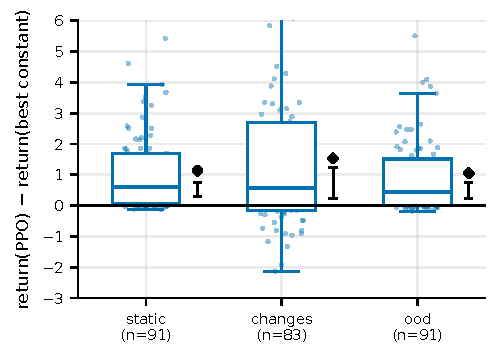
\includegraphics[width=\columnwidth]{fig_paired_conf.pdf}
\caption{Simulation, confirmatory seeds 60000--60099, feasible scenarios: paired return difference of the validation-selected residual PPO (v3) to the best constant, per regime. Box: median and interquartile range; points: every scenario; right of each box: median with $95\,\%$ bootstrap interval (bar) and mean (diamond). Positive is better than the constant.}
\label{fig:paired}\end{figure}

\subsection{How much of the oracle headroom is captured?}\label{sec:headroom}
The hindsight oracle improves on the best constant by $\ConfThreeStaticOrcAbs$, $\ConfThreeChangesOrcAbs$ and $\ConfThreeOodOrcAbs$ mean return in the three regimes ($\ConfThreeStaticOrcPct$, $\ConfThreeChangesOrcPct$ and $\ConfThreeOodOrcPct\,\%$ of $|$return$|$). The selected residual PPO captures $\ConfThreeStaticCap$, $\ConfThreeChangesCap$ and $\ConfThreeOodCap\,\%$ of that headroom; averaged over the three training seeds it captures $\ConfThreeStaticCapMean$, $\ConfThreeChangesCapMean$ and $\ConfThreeOodCapMean\,\%$, and one seed captures less than nothing in the changes regime (Fig.~\ref{fig:headroom}). The learned policy is therefore far from the ceiling for a scenario-aware tuner, most clearly when the payload and target change.

\begin{figure}[t]\centering
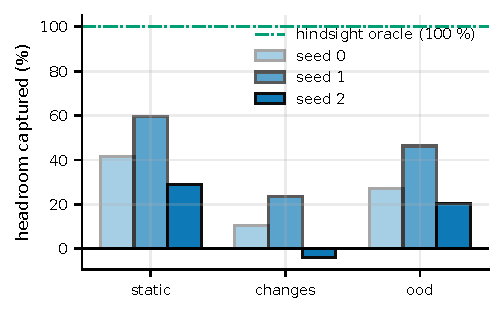
\includegraphics[width=\columnwidth]{fig_headroom.pdf}
\caption{Simulation, confirmatory seeds: headroom captured per training seed, i.e.\ the mean return gain of the policy over the best constant divided by the gain of the hindsight oracle (dashed line: oracle, $100\,\%$), feasible scenarios.}
\label{fig:headroom}\end{figure}

\subsection{Infeasible scenarios}
Infeasible scenarios (margin $<1$ at any point) are $\ConfThreeStaticNInf$, $\ConfThreeChangesNInf$ and $\ConfThreeOodNInf$ of $100$ in the three regimes on the confirmatory seeds. No controller can hold these targets; the policy is not better than the best constant there (changes regime: mean return $\ConfThreeChangesInfPpo$ against $\ConfThreeChangesInfBase$, oracle $\ConfThreeChangesInfOrc$; Table~\ref{tab:infeasible}). They are excluded from the headline tables.

\begin{table}[t]
\centering
\small
\caption{Infeasible scenarios (torque margin $<1$ at any point), confirmatory seeds 60000--60099: mean return. No controller can hold these targets; differences are not evidence of better control.}
\label{tab:infeasible}
\begin{tabular}{lrrrr}
\toprule
Controller & static & changes & ood & \\
\midrule
Tuned preset & $-$40.4 & $-$92.7 & $-$35.8 & \\
Bandit (one-shot) & $-$38.2 & $-$84.2 & $-$34.9 & \\
Best constant & $-$39.5 & $-$85.5 & $-$35.5 & \\
PPO residual (selected) & $-$38.5 & $-$85.2 & $-$35.0 & \\
Hindsight oracle & $-$37.7 & $-$42.6 & $-$34.7 & \\
\midrule
$n$ infeasible & 9 & 17 & 9 & \\
\bottomrule
\end{tabular}
\end{table}


\subsection{v4: a smaller residual range, and SAC and TD3}\label{sec:v4}
On the unseen seeds $70000$--$70099$ PPO with the smaller range gave median differences of $\VFourPpoStaticMed$ (static) and $\VFourPpoOodMed$ (ood), but seed 0 was worse than the constant in both and the changes regime was inconclusive ($\VFourPpoChangesMed$, mean $\VFourPpoChangesMean$, IQR [$\VFourPpoChangesQone$, $\VFourPpoChangesQthree$]); the benefit is smaller than in v3 and the seed sets differ, so we do not conclude that the smaller range is better or worse. \textbf{SAC is mixed:} in the static regime the selected seed's median difference is $\VFourSacStaticMed$ [$\VFourSacStaticLo$, $\VFourSacStaticHi$], an interval that excludes zero, but the paired Wilcoxon test is not significant (Holm-adjusted $p=\VFourSacStaticSeedAHolm$), the mean is $\VFourSacStaticMean$ and the interquartile range [$\VFourSacStaticQone$, $\VFourSacStaticQthree$] straddles zero; the other two seeds are $\VFourSacStaticSeedBMed$ and $\VFourSacStaticSeedCMed$, and all three SAC seeds are worse than the constant when payload and target change. \textbf{TD3 did not beat the constant} (static median $\VFourTdStaticMed$, changes $\VFourTdChangesMed$). SAC and TD3 selected early checkpoints and degraded afterwards (validation degradation up to $\VFourSacValDegA$ and $\VFourTdValDegB$ return units, against at most $\VFourPpoValDegC$ for PPO). No policy helped in the changes regime in v4 (Table~\ref{tab:v4}, Fig.~\ref{fig:algos}).

\begin{table*}[t]
\centering
\small
\caption{Experiment v4 (smaller residual range; PPO, SAC, TD3), unseen seeds 70000--70099, feasible scenarios. Paired return difference to the best constant for the validation-selected seed: median [95\,\% CI] / mean [95\,\% CI] / IQR, and the three per-seed medians. $p_{\mathrm{Holm}}$ over the secondary family of each algorithm.}
\label{tab:v4}
\begin{tabular}{llrrrr}
\toprule
Algorithm & Regime & $\Delta$ median [95\,\% CI] & $\Delta$ mean [95\,\% CI] & IQR & per-seed medians (s0/s1/s2)\\
\midrule
PPO & static & +0.35 [+0.34, +0.36] & +0.38 [+0.36, +0.40] & [+0.33, +0.39] & $-$0.62 / +0.33 / +0.35\\
 & changes & +0.18 [$-$0.08, +0.43] & $-$0.49 [$-$1.28, +0.18] & [$-$0.52, +0.77] & $-$1.20 / +0.13 / +0.18\\
 & ood & +0.34 [+0.29, +0.36] & +0.31 [+0.14, +0.47] & [+0.25, +0.57] & $-$0.56 / +0.30 / +0.34\\
\midrule
SAC & static & +0.25 [+0.12, +0.32] & +0.05 [$-$0.18, +0.28] & [$-$0.29, +0.41] & +0.25 / +0.08 / $-$0.24\\
 & changes & $-$0.26 [$-$1.14, $-$0.06] & $-$1.57 [$-$2.39, $-$0.86] & [$-$2.37, +0.12] & $-$0.26 / $-$0.97 / $-$1.40\\
 & ood & +0.24 [+0.19, +0.29] & $-$0.03 [$-$0.28, +0.18] & [$-$0.02, +0.37] & +0.24 / +0.07 / $-$0.21\\
\midrule
TD3 & static & $-$0.17 [$-$0.29, +0.09] & +0.17 [$-$0.09, +0.45] & [$-$0.64, +0.54] & $-$1.02 / $-$0.70 / $-$0.17\\
 & changes & $-$2.13 [$-$2.50, $-$1.82] & $-$2.06 [$-$2.91, $-$0.72] & [$-$3.70, $-$1.17] & $-$2.13 / $-$2.38 / $-$1.49\\
 & ood & $-$0.10 [$-$0.26, +0.04] & +0.19 [$-$0.13, +0.54] & [$-$0.66, +0.47] & $-$0.89 / $-$0.70 / $-$0.10\\
\bottomrule
\end{tabular}
\end{table*}


\begin{figure*}[t]\centering
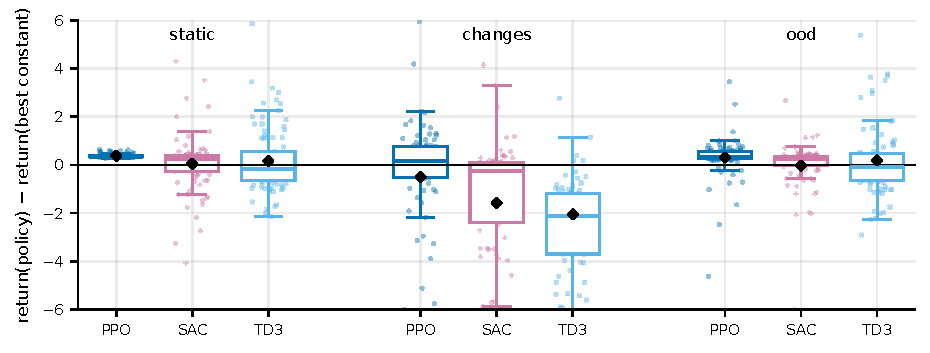
\includegraphics[width=\textwidth]{fig_algos.pdf}
\caption{Simulation, unseen seeds 70000--70099 (v4), feasible scenarios: paired return difference of the validation-selected policy of each algorithm to the best constant, per regime. Box: median and interquartile range, points: scenarios, diamond: mean.}
\label{fig:algos}\end{figure*}

\begin{figure*}[t]\centering
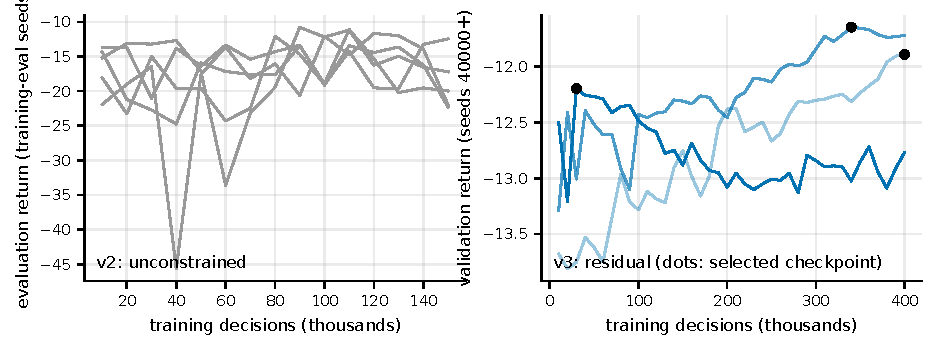
\includegraphics[width=\textwidth]{fig_curves.pdf}
\caption{Simulation. Left: v2 evaluation return on the training-evaluation seeds (five seeds): peak at $60$k--$120$k decisions, then degradation. Right: v3 validation return on seeds 40000+ (three seeds); dots mark the checkpoint selected on validation. The two panels use different evaluation streams and are not the same measurement.}
\label{fig:curves}\end{figure*}

\subsection{Post-hoc check: is the benefit just a better constant?}\label{sec:posthoc}
The learned policies end at gains that vary little across scenarios: in v3 the median final gains are $K_p=\ConfThreeStaticGainKpMed$ ($10$--$90\,\%$ range $\ConfThreeStaticGainKpPlo$--$\ConfThreeStaticGainKpPhi$) and $K_d=\ConfThreeStaticGainKdMed$ in the static regime, against $\ConfThreeStaticGainKpBase$ and $\ConfThreeStaticGainKdBase$ for the best constant; in v4 the PPO gains are almost constant ($K_p=\VFourPpoStaticGainKpMed$, $10$--$90\,\%$ range $\VFourPpoStaticGainKpPlo$--$\VFourPpoStaticGainKpPhi$). This raises the possibility that part or all of the benefit comes from a better constant than the modest search found, not from adaptation. We therefore added, \emph{after} the confirmatory runs and labelled post hoc, two constants derived on validation seeds only: a much larger validation search and the policy's own median gains.
\textbf{[PENDING: results of \texttt{simulation/constant\_sensitivity.py} (\texttt{results/constant\_sensitivity\_v3}); this paragraph and the claim in the abstract must be revised according to them before the draft is polished.]}
